% !Mode\dots ``TeX:UTF-8''
% !TEX root = ../bare_jrnl.tex


\section{Introduction}
\label{sec:intro}


\IEEEPARstart{I}n 1960s, Nobel Prize laureates Jacob and Monod~\cite{Jacob1961Genetic} found that ``Any cell contains a number of regulatory genes that act as switches and can turn one another on and off. If genes can turn one another on and off, then you can have genetic circuits.'' Inspired by these Boolean-type actions in genetic circuits, Boolean networks (\BNs) were firstly proposed by Kauffman for modeling nonlinear and complex biological systems \cite{Kauffman1968Metabolic}. 

{\BNs} are a type of discrete-time dynamical systems which can be represented as directed graphs. In a BN, each node has only two values ``0" and ``1", and they can change in different time points.  For a node $n_i$, we use $n_i(t)$ to denote its value at time $t$.
In general, $n_i(t+1)$ is determined by a logical function of $n_j(t),\ldots,n_p(t)$ if  there are  edges from $n_j,\ldots,n_p$ to $n_i$.  
%The logical operators used in  the logical functions include AND, OR, NO, XOR.  
Some general descriptions of the \BNs\ and their applications to biological systems can be found in~\cite{Kauffman1968Metabolic}. There exists a large number of  systems, both natural and artificial, which are modelled as \BNs, e.g. ~\cite{Akutsu2000Inferring, Shmulevich2002From, Faur2006Dynamical,Green2007The,Lou2010Multi}.

\BNs\ can be naturally extended to Boolean control networks (\BCNs) with external regulations and perturbations~\cite{Ideker2001A}. \BCNs\ have been applied to  various real-life problems. Cases of application can be found in 
structural and functional analysis of signaling and regulatory networks~\cite{Kaufman1999A, Klamt2006A}, 
abduction based drug target discovery~\cite{Biane2017Abduction}, 
and pursuing evasion problems in polygonal environments~\cite{Thunberg2011A}.
%
There are three kinds of nodes in \BCNs:  {\em input-nodes}, {\em state-nodes}  and {\em output-nodes}. At any moment of time each node takes a Boolean value.  The value of an output-node at time point $t$ (where $t\geq 0$)  depends on the values of state-nodes at time $t$, but the value of a  state-node at time point $t+1$  is determined by a  Boolean function of the values of the input-nodes and state-nodes at time point $t$. And these relations between nodes are presented by the updating rules of \BCN.  However,  we can only control the  values of the input-nodes and observe those of the output-nodes. We cannot observe how the values of the state-nodes change from time to time.
%Therefore, it is important to find a way to determine the initial values of the state-nodes at $0$ after observing a sequence of values of  input-nodes and their corresponding  values of the output-nodes. This is in general known as the {\em observability} of a \BCN.

The identification of \BCNs\ was proposed in~\cite{Cheng2011Identification}. It is about how to determine the updating rules of a \BCN\ from the values of  input-nodes  and output-nodes at a sequence of time points $0,\ldots, k$. And it is an important topic, for example, we may be interested in the updating rules of a \BCN\ which present a real celluar network. 

%Observability is one of the two basic  properties related to  the control-theoretic problems of \BCNs. The other is known as {\em controllability}. The work in ~\cite{Akutsu2007Control} shows that the problem of determining the controllability of \BCNs\ is {NP}-hard. Moreover, it  points out that ``One of the major goals of systems biology is to develop a control theory for complex biological systems.''  Since then, research on  controllability and observability of \BNs\ and \BCNs\ has drawn a great attention, e.g. \cite{cheng2009controllability, Zhao2010Input, Cheng2011Identification, Cheng2011Analysis} and \cite{Fornasini2013Observability}. %There, it is further noted that the controllability and observability are the basic control-theoretic problems of \BCNs. % Among these studies, \emph{semi-tensor product} (\STP) is one of useful tools to deal with  

 %The concept of observability was first proposed in~\cite{cheng2009controllability}. It is mainly about how  to determine  the values of the  state-nodes  of a \BCN\  at time $0$ from the values of  input-nodes  and output-nodes at a sequence of time points $0,\ldots, k$. After that, four types of observability have been investigated in the literature, together with their corresponding determining algorithms, which we will discuss below.

\begin{figure}[!t]
      \centering
      \framebox{\parbox{3in}{
		\centerline{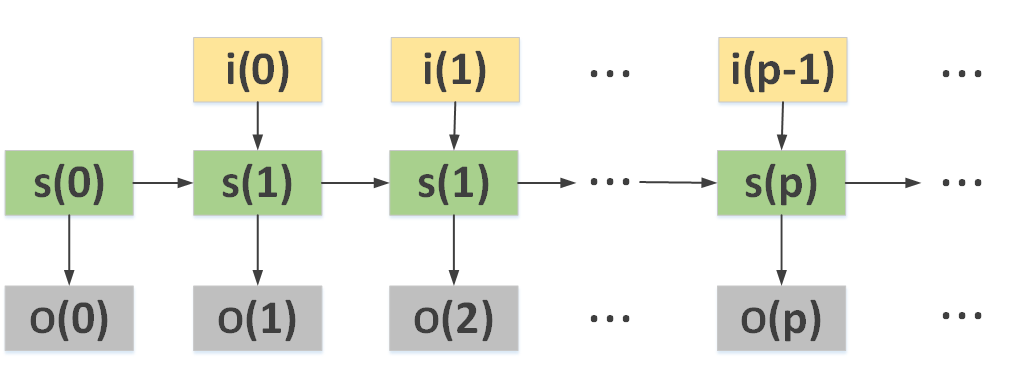
\includegraphics[scale=0.17]{figures/Fig10.png}}
	}}
      
      \caption{The relationship of inputs, states and outputs.}
      \label{fig:10}
  \end{figure}

Given a \BCN\ with $\ell$ input-nodes $(\mathsf{i}_1,\ldots, \mathsf{i}_\ell)$, $m$ state-nodes $(\mathsf{s}_1,\ldots, \mathsf{s}_m)$ and $n$ output notes  $(\mathsf{o}_1,\ldots, \mathsf{o}_n)$,  we use an {\em input vector} $\mathsf{i}(t)=(\mathsf{i}_1(t)\ldots\mathsf{i}_\ell (t))$, a {\em state vector} $\mathsf{s}(t)=(\mathsf{s}_1(t), \ldots \mathsf{s}_m(t))$ and an {\em output  vector} $\mathsf{o}(t)=(\mathsf{o}_1(t) \ldots \mathsf{o}_n(t))$  to represent an assignment of Boolean values to the  input-nodes, state-nodes and  output-nodes at $t$, respectively.  We call them an {\em input}, a {\em state} and an {\em output} of the \BCN\ at time time $t$. As  illusreated by Fig.~\ref{fig:10},  the state $\mathsf{s}(t+1)$ at time $t+1$ is determined by the input   $\mathsf{i}(t)$ and state $\mathsf{s}(t)$ at $t$  and the output   $\mathsf{o}(t)$ by the state  $\mathsf{s}(t)$.  We call a state $\mathsf{s}(0)$ at time $0$ an {\em initial state}. Thus, for any $k>0$, the state sequence  $\mathsf{s}(1),\ldots, \mathsf{s}(k)$ and the output sequence $\mathsf{o}(0)\ldots, \mathsf{o}(k)$ are  determined by an  input sequence $\mathsf{i}(0),\ldots, \mathsf{i}(k-1)$ and initial state $\mathsf{s}(0)$.
%That is for a given  \BCN\  $\BB$,  $\mathsf{o}(0)\mathsf{o}(1)\ldots\mathsf{o}(k)$ is decide by $\mathsf{s}(0)$ and the sequence $\mathsf{i}(0)\mathsf{i}(1)\ldots\mathsf{i}(k-1)$. 
%
The identifiability of \BCNs\ can thus be described as follows. 

{\em Identifiability}:
A \BCN\ $\BB$ is identifiable if its updating rules can be determined via its input-output data $\mathsf{i}(0),\mathsf{i}(1),\ldots, \mathsf{i}(k-1)$ and $\mathsf{o}(0)\ldots, \mathsf{o}(k)$.
Precisely speaking, there is an input sequence $\mathsf{I}=\mathsf{i}(0),\mathsf{i}(1),\ldots, \mathsf{i}(k-1)$ for some $k>0$ which produces output sequence $\mathsf{O}=\mathsf{o}(0)\ldots, \mathsf{o}(k)$, such that the updating rules of $\BB$ can be determined via $\mathsf{I}$ and $\mathsf{O}$ \cite{Cheng2011Identification}.
%\begin{enumerate}
%\item The  {\bf type-I}  observability was proposed in 2009 \cite{cheng2009controllability}. It states that a \BCN\ $\BB$ is observable if for any initial state   $\mathsf{s}(0)$ there exists an input sequence  $\mathsf{i}(0),\mathsf{i}(1),\ldots,\mathsf{i}(k-1)$ which can  distinguish $\mathsf{s}(0)$ from any other initial state $s'(0)$. That is,  given an initial state $\mathsf{s}(0)$, there is an input sequence $\mathsf{I}=\mathsf{i}(0),\mathsf{i}(1),\ldots,\mathsf{i}(k-1)$ for some $k>0$ such that  for any  $\mathsf{s}'(0)$ which is different from $\mathsf{s}(0)$, the output sequence  $\mathsf{O}=\mathsf{o}(0),\mathsf{o}(1),\ldots,\mathsf{o}(k)$ produced by  $\mathsf{s}(0)$ and $\mathsf{I}$ is different the output sequence  $\mathsf{O}'=\mathsf{o}'(0),\mathsf{o}'(1),\ldots, \mathsf{o}'(k)$ produced by  $\mathsf{s}'(0)$ and $\mathsf{I}$.

%\item The  {\bf type-II} observability was proposed in 2010 \cite{Zhao2010Input}. It states that a \BCN\ $\BB$ is observable if for every two different initial states $\mathsf{s}(0)$ and $\mathsf{s}'(0)$, there exists an input sequence $\mathsf{i}(0),\mathsf{i}(1),\ldots, \mathsf{i}(k-1)$ that can distinguish $\mathsf{s}(0)$ and $\mathsf{s}'(0)$. More precisely speaking,  for any pair of different initial  $\mathsf{s}(0)$ and $\mathsf{s}'(0)$, there exists an input sequence  $\mathsf{i}(0),\mathsf{i}(1),\ldots,\mathsf{i}(k-1)$ for some $k>0$ such that the output sequences $\mathsf{o}(0),\mathsf{o}(1),\ldots,\mathsf{o}(k)$ and  $\mathsf{o}'(0),\mathsf{o}'(1),\ldots,\mathsf{o}'(k)$ corresponding to  the different initial states  $\mathsf{s}(0)$ and $\mathsf{s}'(0)$, respectively, are different.
	
%\item The  {\bf type-III} observability was proposed in 2011 \cite{Cheng2011Identification}.  It states that a \BCN\ $\BB$ is observable if there is an input sequence $\mathsf{i}(0),\mathsf{i}(1),\ldots, \mathsf{i}(k-1)$ that distinguishes every pair of different initial states. This means that in $\BB$, there exists an input sequence  $\mathsf{i}(0),\mathsf{i}(1), \ldots,\mathsf{i}(k-1)$ for some $k>0$ such that for any two different initial states $\mathsf{s}(0)$ and $\mathsf{s}'(0)$, the output sequence $\mathsf{o}(0),\mathsf{o}(1), \ldots, \mathsf{o}(k)$  corresponding to  $\mathsf{s}(0)$  is different from the output sequence  $\mathsf{o}'(0),\mathsf{o}'(1),\ldots, \mathsf{o}'(k)$ corresponding to $\mathsf{s}'(0)$.
%\JP{Please don't change notations. Stick to $s(0)$ and $s'(0)$. $\mathsf{s}^{x}(0)$ and $\mathsf{s}^{y}(0)$ are somehow strange.}
	
%\item  The  {\bf type-IV}  observability was  proposed in 2013 \cite{Fornasini2013Observability}. It states that a \BCN\ $\BB$ is observable if every sufficient long $\mathsf{i}(0)\mathsf{i}(1),\ldots,\mathsf{i}(k-1)$ genertaes different output sequences  from different initial states. Precisely speaking, there is a big enough number $M$, for every  input sequence $\mathsf{i}(0),\mathsf{i}(1),\ldots, \mathsf{i}(k-1)$ which is not shorter than $M$, the output sequences $\mathsf{o}(0), \mathsf{o}(1), \ldots, \mathsf{o}(k)$ and  $\mathsf{o}'(0), \mathsf{o}'(1), \ldots, \mathsf{o}'(k)$ produced by the inout sequence from every two different initial states $\mathsf{s}(0)$ and $\mathsf{s}'(0)$, respectively, are different.
%\end{enumerate}
 We will give the formal definition of identifiability in Section~\ref{sec:pre}. And in this paper \cite{Cheng2011Identification}, author claims that a \BCN\ is identifiable iff it is controllable and observable. The controllability and observability are described as follows. 
 %\JP{So far, I don't see a clear difference among the first three types from the above description.}

{\em Controllability}: A \BCN\ $\BB$ is controllable if for any initial state $\mathsf{s}(0)$ and destination state $\mathsf{s}(k)$, there exists an input sequence $\mathsf{i}(0),\mathsf{i}(1),\ldots,\mathsf{i}(k-1)$ for some $k>0$, such that the state sequence $\mathsf{s}(1),\ldots, \mathsf{s}(k)$ can be produced by $\mathsf{I}$.

{\em Observability}:
A \BCN\ $\BB$ is observable if there is an input sequence $\mathsf{i}(0),\mathsf{i}(1),\ldots, \mathsf{i}(k-1)$ that distinguishes every pair of different initial states. This means that in $\BB$, there exists an input sequence  $\mathsf{i}(0),\mathsf{i}(1), \ldots,\mathsf{i}(k-1)$ for some $k>0$ such that for any two different initial states $\mathsf{s}(0)$ and $\mathsf{s}'(0)$, the output sequence $\mathsf{o}(0),\mathsf{o}(1), \ldots, \mathsf{o}(k)$  corresponding to  $\mathsf{s}(0)$  is different from the output sequence  $\mathsf{o}'(0),\mathsf{o}'(1),\ldots, \mathsf{o}'(k)$ corresponding to $\mathsf{s}'(0)$.

 We will give the formal definitions of them in Section~\ref{sec:pre}. The identification problem of \BCNs\ requires \BCNs\ to satisfy the observability because we need to determine the initial state of \BCNs\ if we want to identify their updating rules. And when a \BCN\ $\BB$ is observable them we can determine its initial state $\mathsf{s}(0)$ by the following algorithm.

%Algorithms exist for deciding if a \BCN\ has one of these four types of observability. Now we explain how each type of observability give rise a algorithm to determine the initial state of a \BCN\ by providing input sequences and observing their correspodning output sequences.

%\JP{Here, you need an introductory sentence on why algorithms are needed.}
%Four types of observability develop different algorithms to determine $\mathsf{s}(0)$ of \BCN. 

%后面能用到
%

%Assume a \BCN\ $\BB$  with {\bf type-I}  observability. At time $0$ we can  obtain $\mathsf{S}(0)$ of $\BB$ by $\mathsf{o}(0)$. Then, for each initial state $\mathsf{s}'(0)\in \mathsf{S}(0)$, there is a correspdining input sequence $\mathsf{i}'(0),\mathsf{i}'(1),\ldots, \mathsf{i}'(k-1)$ for which the corresoning output sequnece $\mathsf{o}'(0),\mathsf{o}'(1),\ldots,\mathsf{o}'(k)$ is different from the output sequence $\mathsf{o}''(0),\mathsf{o}''(1),\ldots,\mathsf{o}''(k)$ for a different initial state $\mathsf{s}''(0)\in \mathsf{S}(0)$ with the same inpout sequnece. Thus, we have foloiwng procedure to determe its initial state $\mathsf{s}(0)$.
%\begin{description}
	%\item[Step 1] Set variable $\mathsf{S}$ be set to $\mathsf{S}(0)$.
	%\item[Step 2] Choose a initial state $\mathsf{s}'(0)$ from $\mathsf{S}$, input to the \BCN\ $\BB$ with the input sequence $\mathsf{i}'(0),\mathsf{i}'(1),\ldots, \mathsf{i}'(k-1)$, which distinguish $\mathsf{s}'(0)$ from other initial states, and run $\BB$ to generate the output sequence $\mathsf{o}(0),\mathsf{o}(1),\ldots,\mathsf{o}(k)$.
	%\item[Step 3] If the ouput sequence $\mathsf{o}(0),\mathsf{o}(1),\ldots,\mathsf{o}(k)$ is the same as the output sequence $\mathsf{o}'(0),\mathsf{o}'(1),\ldots,\mathsf{o}'(k)$ for $\mathsf{s}'(0)$, then return $\mathsf{s}'(0)$ as the initial state of $\BB$. Otherwise, set $\mathsf{S}=\mathsf{S}-\{\mathsf{s}'(0)\}$ by removing $\mathsf{s}'(0)$ from the $\mathsf{S}$, and go to Step 2.
	
%\end{description}

% Assume a \BCN\ $\BB$  with {\bf type-II}  observability. At time $0$ we can  obtain $\mathsf{S}(0)$ of $\BB$ by $\mathsf{o}(0)$. Then, for every two different initial states $\mathsf{s}'(0), \mathsf{s}''(0)\in \mathsf{S}(0)$ of $\BB$, there is a correspdining input sequence $\mathsf{i}'(0),\mathsf{i}'(1),\ldots, \mathsf{i}'(k-1)$ for which the corresoning output sequnece $\mathsf{o}'(0),\mathsf{o}'(1),\ldots,\mathsf{o}'(k)$ is different from the output sequence $\mathsf{o}''(0),\mathsf{o}''(1),\ldots,\mathsf{o}''(k)$ for the initial state $\mathsf{s}''(0)$ with the same inpout sequnece. Thus, we have foloiwng procedure to determe its initial state $\mathsf{s}(0)$.
%\begin{description}
	%\item[Step 1]  Set variable $\mathsf{S}$ be set to $\mathsf{S}(0)$.
	%\item[Step 2] Choose two initial states $\mathsf{s}'(0)$ and $\mathsf{s}''(0)$ from $\mathsf{S}$, input to the \BCN\ $\BB$ with the input sequence $\mathsf{i}'(0),\mathsf{i}'(1),\ldots, \mathsf{i}'(k-1)$, which distinguish $\mathsf{s}'(0)$ and $\mathsf{s}''(0)$, and run $\BB$ to generate the output sequence $\mathsf{o}(0),\mathsf{o}(1),\ldots,\mathsf{o}(k)$.
	%\item[Step 3] With the input sequence $\mathsf{i}'(0),\mathsf{i}'(1),\ldots, \mathsf{i}'(k-1)$ and output sequence $\mathsf{o}(0),\mathsf{o}(1),\ldots,\mathsf{o}(k)$, we can get the new $\mathsf{S}(0)$ ($t=k>0$).
	%\item[Step 4] Set $\mathsf{S}=\mathsf{S}\cap\mathsf{S}(0)$ by the intersection of $\mathsf{S}(0)$ and $\mathsf{S}$. If the cardinal number of $\mathsf{S}$ equal to $0$, then return the $\mathsf{s}'(0)$ belonging to $\mathsf{S}$ as the initial state of $\BB$. Otherwise, go to Step 2.
%\end{description}

Assume a \BCN\ $\BB$  with the observability. Then, there is an input sequence $\mathsf{i}(0),\mathsf{i}(1),\ldots, \mathsf{i}(k-1)$ that distinguishes every pair of different initial states $\mathsf{s}'(0), \mathsf{s}''(0)$ of $\BB$. Thus, we have foloiwng procedure to determe its initial state $\mathsf{s}(0)$.

 \begin{description}
	\item[Step 1]  Input to the \BCN\ $\BB$ with the input sequence $\mathsf{i}(0),\mathsf{i}(1),\ldots, \mathsf{i}(k-1)$, which distinguish every pair of different initial states $\mathsf{s}'(0)$ and $\mathsf{s}''(0)$, and run $\BB$ to generate the output sequence $\mathsf{o}(0),\mathsf{o}(1),\ldots,\mathsf{o}(k)$.
	\item[Step 2] Return $\mathsf{s}'(0)$ which produces $\mathsf{o}(0),\mathsf{o}(1),\ldots,\mathsf{o}(k)$ as the initial state of $\BB$ 
\end{description}

%Assume a \BCN\ $\BB$  with {\bf type-IV}  observability. Then, there is a big enough number $M$, for every  input sequence $\mathsf{i}(0),\mathsf{i}(1),\ldots, \mathsf{i}(k-1)$ which is not shorter than $M$,  $\mathsf{i}(0),\mathsf{i}(1),\ldots, \mathsf{i}(k-1)$ distinguishes every pair of different initial states $\mathsf{s}'(0), \mathsf{s}''(0)$ of $\BB$. Thus, we have foloiwng procedure to determe its initial state $\mathsf{s}(0)$.

% \begin{description}
	%\item[Step 1]  Input to the \BCN\ $\BB$ with the input sequence $\mathsf{i}'(0),\mathsf{i}'(1),\ldots, \mathsf{i}'(k-1)$,  which is not shorter than $M$, and run $\BB$ to generate the output sequence $\mathsf{o}(0),\mathsf{o}(1),\ldots,\mathsf{o}(k)$.
	%\item[Step 2] Return $\mathsf{s}'(0)$ which produces $\mathsf{o}(0),\mathsf{o}(1),\ldots,\mathsf{o}(k)$ as the initial state of $\BB$ 
%\end{description}
%{\color{red} (13)}

%Loosely speaking, different applications require different algorithms to determine $\mathsf{s}(0)$, and the four types of observability present whether a \BCN\ can be determined by these four algorithms respectively. In the algorithms corresponding to {\bf type-I} and {\bf type-II} observability, it requires the $\mathsf{s}(0)$ of \BCN\ can be reset because we need to repeat the Step 2. Thus when the initial state of \BCN\ can be reset, we use these two ways to determine $\mathsf{s}(0)$. The {\bf type-IV} observability is proposed to research the reconstructibility of \BCN. The {\bf type-III} observability is proposed to research the identification of \BCN. 

%Moreover, in the identification problem of \BCNs, a \BCN\ is identifiable iff it is controllable and its $\mathsf{s}(0)$ can be determined when $\mathsf{s}(0)$ cannot be reset \cite{Cheng2011Identification}. And in this paper \cite{Cheng2011Identification}, author regards the {\bf type-III} observability as the necessary and sufficient condition of determining $\mathsf{s}(0)$ when $\mathsf{s}(0)$ cannot be reset. %And the second observability is the necessary and sufficient condition of determining $\mathsf{s}(0)$ by taking the determining procedure once. 
%\JP{What applications?}

While, in this paper, we propose a new algorithm to determine $\mathsf{s}(0)$. %address the necessary and sufficient condition of determining $\mathsf{s}(0)$ by taking the determining process once to make \BCN\ be able to apply to more applications.
%\JP{Here, `necessary and sufficient condition' appears for the first time. What are their precise definitions?}
%Naturally there is a procedure to determine $\mathsf{s}(0)$  which is described as follows.
%\JP{Why in this way it can be applied to more applications?}
%It enriches the control-theory of \BCNs, it can help us determine the $\mathsf{s}(0)$ of some \BCNs\ which can not be determined before.
Let $\mathsf{S}(0)$ denote the set of possible valuations of $\mathsf{s}(0)$. We obtain it by the information about the input and output of \BCN. When $t=0$, assume $\mathsf{o}(0)$ is the initial output of the \BCN, then for every $\mathsf{s}'(0)\in\mathsf{S}(0)$, $\mathsf{s}'(0)$ produces $\mathsf{o}(0)$. When $t>0$, assume $\mathsf{I}=\mathsf{i}(0),\mathsf{i}(1),\ldots,\mathsf{i}(t-1)$ and $\mathsf{O}=\mathsf{o}(0),\mathsf{o}(1),\ldots,\mathsf{o}(t)$ present the input sequence and the output sequence of \BCN, respectively, then for every $\mathsf{s}'(0)\in\mathsf{S}(0)$, $\mathsf{s}'(0)$ and $\mathsf{I}$  produce  $\mathsf{O}$. Let $\mathsf{S}(t)$ denote the set of possible valuations of $\mathsf{s}(t)$, then it is produced by $\mathsf{S}(0)$ and $\mathsf{I}$.
The new algorithm is described as follows. 

%\begin{problem}
%\label{pro:1}
%For a given \BCN\ $\BB$, whether its initial state $\mathsf{s}(0)$ can be determined by carrying on determining procedure once?
%\end{problem}

%Although, these four existing notions of observability can help us study some information about $\mathsf{s}(0)$ we need. 
%The problem means that whether the $\mathsf{s}(0)$ can be determined if the determining procedure can do at most once. %only third and fourth ones  can  determine the $\mathsf{s}(0)$ of \BCNs.
%Only third and fourth notions of observability can help us solve the {\em Problem~\ref{pro:1}}.
% What is more, in the third observability, a \BCN\ is observable iff there is an input sequence that determines its initial state $\mathsf{s}(0)$. Thus its condition is very strong, and the condition of fourth observability is even stronger.
%However, 
%Let $\mathsf{S}(t)$ denote the set of possible valuations of $\mathsf{s}(t)$. Then naturally there is a procedure which is described as follows.
%We find that to determine $\mathsf{s}(0)$ by taking the determining procedure once we only need to complete the following procedure. 

%Informly, the procedure of our  online observability as follows. 
 %Then $\mathsf{S}(t)$ can be derived by the output sequence $\mathsf{o}(0)\mathsf{o}(1)\ldots\mathsf{o}(t)$, input sequence $\mathsf{i}(0)\mathsf{i}(1)\ldots\mathsf{i}(t-1)$ and updating rules of $\BB$.
 
 %\tl{can you make this a proper algorithm?}\gs{I have corrected this one.}
\begin{description}
	\item[Step 1]  Set variable $\mathsf{S}$ be set to $\mathsf{S}(t)$ ($t=0$).
	\item[Step 2] Input to the \BCN\ $\BB$ with the an $\mathsf{i}$ which would not make every two distinct $\mathsf{s}'$, $\mathsf{s}''$$\in$ $\mathsf{S}$ become the same state after affected by $\mathsf{i}$, and run $\BB$ to generate the new output $\mathsf{o}(t)$.
	\item[Step 3] Get the new $\mathsf{S}(t)$ and $\mathsf{S}(0)$ based on the input sequence $\mathsf{i}(0),\mathsf{i}(1),\ldots, \mathsf{i}(t-1)$ and output sequence $\mathsf{o}(0),\mathsf{o}(1),\ldots,\mathsf{o}(t)$ we have collected so far.
	\item[Step 4] If the cardinal number of $\mathsf{S}(0)$ equal to $0$, then we return the $\mathsf{s}'(0)$ belonging to $\mathsf{S}(0)$ as the initial state of $\BB$. Otherwise, set $\mathsf{S}=\mathsf{S}(t)$ by the $\mathsf{S}(t)$, and go to Step 2.
\end{description}

%In the third observability, we can finish this procedure, thus we can determine the initial state \State$(0)$ for a \BCN. What is more, 


%Such that, the requirement for a \BCN\ to determine \State$(0)$ would be easist to satisfy. 
%{\color{red} (13)} 
We propose a new type of observability named {\em online observability} which states that a \BCN\ is observable if its \State$(0)$ can be determined by this algorithm. Its formal definition will be presented in Section~\ref{sec:online}.  We call this observability online observability, because we observe $\mathsf{o}(t)$ of \BCN\ and choose $\mathsf{i}(t)$ based on the information we have collected so far at every time $t$. 

In contrast, in the observability proposed in \cite{Cheng2011Identification}, we determine $\mathsf{s}(0)$ of \BCN\ by its recorded $\mathsf{o}(0)\mathsf{o}(1)\ldots\mathsf{o}(k)$ after we input $\mathsf{i}(0)\mathsf{i}(1)\ldots\mathsf{i}(k-1)$, and  we do not interfere with \BCN\ except for the logging of its inputs and outputs, thus we call it {\em offline observability} \cite{Cassar2017A}.
 
  And the online observability is the necessary and sufficient condition of determining $\mathsf{s}(0)$ when $\mathsf{s}(0)$ can not be reset. This proposition will be supported by the formal definition of  online observability.  Thus we can research the identification problem of \BCNs\ by this type of observability instead of the offline observability.


\JP{It is very unclear why we need this new notion and why it is supposed to be better.}
\JP{In general, the introduction lacks of a good motivation for the current research.
Can you somehow re-structure the introduction?
1. What is the context of this paper?
2. What exactly is the research problem and why it is important?
3. What are the existing solutions and why they are not sufficient?
4. What is your new solution and its main idea?
5. Why is your new solution better?
6. Any evidence to support your claim?}

 %{\color{red} (13)}

In addition to giving the formal definition of online observability, we also provide a determination algorithm for it. To this end, we firstly define {\em input-labelled graphs} for BCNs, which consist of sets of states of \BCNs\ producing the same outputs, and transitions between the sets. And then, we propose the determination algorithm based on the input-labelled graph.

Thus in this paper we make the following contributions.

%Then, in this paper we make the following contributions. 
\medskip\noindent
{\bf Contributions.}
Firstly, we propose and formally define the online observability to help us further researching the identification problem of \BCNs. % to address the necessary and sufficient condition of determining $\mathsf{s}(0)$ by taking the determining procedure once. %It enriches the control-theory of \BCNs. 
Secondly, we also provide a determination algorithm for the online observability. %Finally, we present some optimization brought by the online observability. Including the means to find shortest path and the approach to avoid entering critical states in the process of determining the initial states of \BCNs.  These optimization further explain the advantages of online observability of \BCNs. 

\medskip\noindent
{\bf Plan of the paper.}
The remainder of this paper is organized as follows.
 {\em Section \ref{sec:pre}} introduces necessary preliminaries about \BCNs, including the definition, four existing types of observability and the identification of \BCNs. {\em Section \ref{sec:online}} presents the definition of online observability of \BCNs. {\em Section \ref{sec:deter}} presents the determination algorithm for online observability. 
% {\em Section \ref{sec:app}} talks about some optimization brought by the online observability of \BCNs. 
 {\em Section \ref{sec:con}} ends up with the introduction of our future work.

%==============================================================================================================